% ===========================================================================
% Numerical verification
% ===========================================================================

\section{Numerical verification}
\label{sec:numerical}

We first test \texttt{diffusionsde} on two stochastic systems for which independent numerical reference solutions are available. The examples are chosen to separate increasingly difficult aspects of the modelling problem. The Ornstein--Uhlenbeck process is linear and Gaussian, with known stationary statistics, and therefore provides a controlled test of whether the model reproduces stochastic fluctuations and temporal correlations. The driven Duffing oscillator introduces nonlinear dynamics, a bistable potential, coloured forcing, and an initial velocity that is deliberately hidden from the diffusion model. It therefore tests whether the model can represent a nontrivial conditional distribution rather than reconstructing a trajectory from a fully specified state.

The magnetic systems considered in Section~\ref{sec:experimental} extend this hierarchy further, replacing low-dimensional stochastic equations by stochastic micromagnetic simulations and, finally, experimental measurements for which no complete dynamical model is assumed.

% ---------------------------------------------------------------------------
\subsection{Ornstein--Uhlenbeck process}
\label{ssec:ou}

The Ornstein--Uhlenbeck (OU) process \cite{uhlenbeck1930} is the simplest stochastic system considered in this work. It obeys
\begin{equation}
    \mathrm{d}q
    =
    -\theta q\,\mathrm{d}t
    +
    \sqrt{2D}\,\mathrm{d}W,
    \label{eq:ou}
\end{equation}
where $\theta>0$ is the relaxation rate and $D>0$ is the diffusion coefficient. Its stationary distribution and normalised autocorrelation are
\begin{equation}
    q
    \sim
    \Normal\!\left(0,\frac{D}{\theta}\right),
    \qquad
    \rho(\tau)
    =
    \exp(-\theta|\tau|).
    \label{eq:ou_continuous_stationary}
\end{equation}
The parameters $D$ and $\theta$ therefore control different properties of the trajectories: $D/\theta$ determines their stationary variance, while $\theta^{-1}$ sets the correlation time. The OU process consequently provides a useful test that the diffusion model has learnt more than the marginal scale of the data.

Reference trajectories are generated using Euler--Maruyama,
\begin{equation}
    q_{n+1}
    =
    (1-\theta\Delta t)q_n
    +
    \sqrt{2D\Delta t}\,z_n,
    \qquad
    z_n\sim\Normal(0,1).
    \label{eq:ou_euler_update}
\end{equation}
At finite $\Delta t$, the corresponding discrete process has stationary variance and lag-$h$ autocorrelation
\begin{equation}
    \operatorname{Var}(q_n)
    =
    \frac{2D\Delta t}
    {1-(1-\theta\Delta t)^2},
    \qquad
    \rho_\Delta(h)
    =
    (1-\theta\Delta t)^h,
    \label{eq:ou_discrete_stationary}
\end{equation}
respectively. These approach Eq.~\eqref{eq:ou_continuous_stationary} as $\Delta t\rightarrow0$.

For the dataset, we sample $\theta\sim\mathcal{U}(0.8,3.0)$ and $D\sim\mathcal{U}(0.1,1.5)$. The training and held-out datasets contain 512 and 128 trajectories, respectively. Both $\theta$ and $D$ are supplied to the diffusion model as conditioning variables. Trajectories and conditioning variables are standardised using statistics calculated from the training set. The model is trained with $N_K=1000$ diffusion levels and generated using around 128 deterministic DDIM steps. 

The OU process is non-trivial for the diffusion model: the trajectories are inherently stochastic, and the diffusion model must learn to `denoise' a standard Gaussian distribution to a Gaussian distribution with variance $D/\theta$ and temporal correlations set by $\theta$. \textcolor{red}{Figure [X] shows the a comparison (?) as a function of the number of DDIM steps.}

The held-out parameter pairs are not used during training. We generate one trajectory for each held-out pair $(\theta,D)$ and compare the resulting ensemble with the corresponding numerical reference ensemble. This test therefore measures interpolation across the two-dimensional parameter distribution rather than repeated sampling at a single fixed parameter pair.

Figure~\ref{fig:ou_trajectories} shows representative trajectories. The generated ensemble reproduces the irregular, correlated fluctuations of the reference process and spans a comparable range of amplitudes. No individual generated trajectory is expected to reproduce an individual numerical trajectory: the target of the model is the conditional trajectory distribution.

\begin{figure}[t]
    \centering
    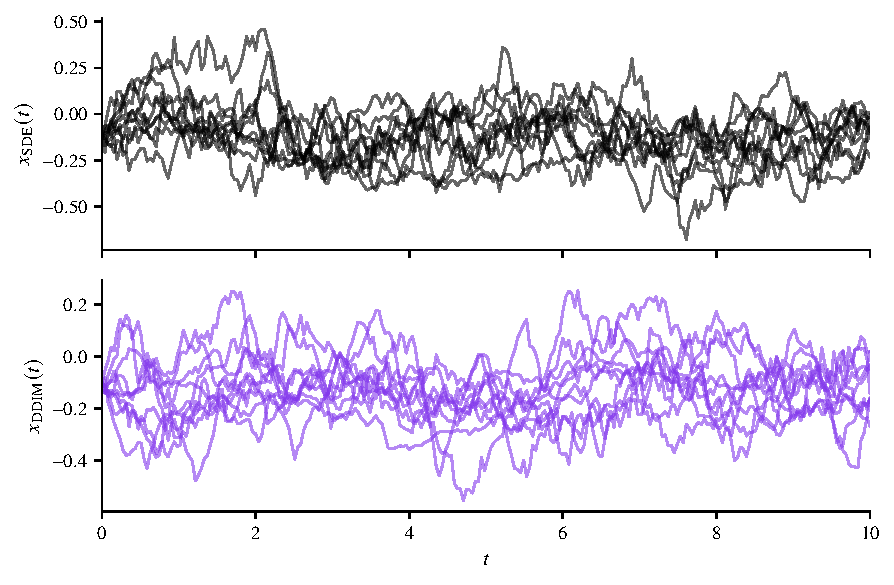
\includegraphics[width=\textwidth]{../ou_trajectories.pdf}
    \caption{
    Representative held-out Ornstein--Uhlenbeck trajectories generated by
    Euler--Maruyama (top) and by the trained diffusion model using deterministic
    DDIM sampling (bottom).
    }
    \label{fig:ou_trajectories}
\end{figure}

A more informative comparison is provided by the ensemble statistics in Fig.~\ref{fig:ou_statistics}. The generated and reference time-dependent means follow one another closely throughout the sampled interval, and the corresponding one-standard-deviation envelopes have similar widths. The diffusion model also reproduces the overall time dependence of the ensemble variance.

\begin{figure}[t]
    \centering
    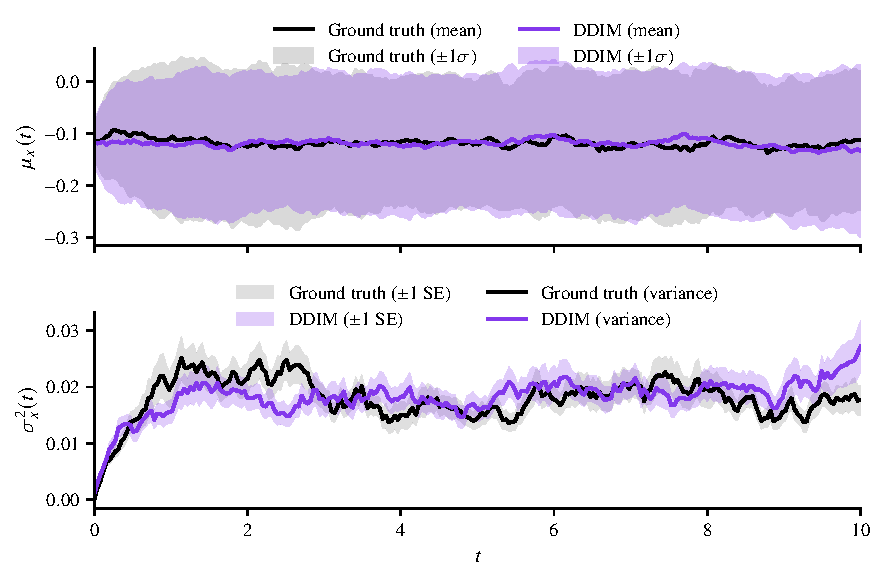
\includegraphics[width=\textwidth]{../ou_statistics.pdf}
    \caption{
    Ensemble statistics for held-out Ornstein--Uhlenbeck trajectories.
    The upper panel compares the time-dependent mean and one-standard-deviation
    interval of the numerical reference and DDIM-generated ensembles. The lower
    panel compares their time-dependent variances; shaded regions indicate the
    corresponding uncertainty in the estimated variance. The diffusion model
    reproduces both the mean response and the scale of the stochastic
    fluctuations, with modest discrepancies in the variance.
    }
    \label{fig:ou_statistics}
\end{figure}

The OU example therefore tests the basic requirement of the method: a conditional generative surrogate should reproduce the statistical behaviour of a stochastic process over parameter values that were not used for fitting. Because exact expressions for the stationary variance and autocorrelation are available, this system also permits more stringent quantitative tests than the more complicated examples considered below.

\textcolor{red}{Need to add more comparison to analytic results}

% TODO: Add direct comparisons of generated variance and correlation time with
% Eq.~\eqref{eq:ou_discrete_stationary} over held-out values of (theta,D).
% This would turn the OU case into a genuinely quantitative analytic benchmark.

% ---------------------------------------------------------------------------
\subsection{Driven Duffing oscillator}
\label{ssec:duffing}

The second numerical example is a periodically driven Duffing oscillator subject to both white and coloured stochastic forcing. Compared with the OU process, this system introduces nonlinear dynamics and a bistable potential, while retaining a well-defined numerical reference model.

Introducing the velocity $v$ and an auxiliary Ornstein--Uhlenbeck variable $\xi$ for the coloured force gives
\begin{align}
    \mathrm{d}q
    &=
    v\,\mathrm{d}t,
    \label{eq:duffing_q}
    \\
    \mathrm{d}v
    &=
    \left[
        -\mu v
        -\alpha_{\mathrm D}q
        -\beta_{\mathrm D}q^3
        +\gamma\cos(\Omega t)
        +\xi
    \right]\mathrm{d}t
    +
    \sqrt{2\mu\Theta}\,\mathrm{d}W_1,
    \label{eq:duffing_v}
    \\
    \mathrm{d}\xi
    &=
    -\frac{\xi}{\tau_c}\,\mathrm{d}t
    +
    \sqrt{\frac{2D_\xi}{\tau_c}}\,\mathrm{d}W_2.
    \label{eq:duffing_colour}
\end{align}
The Wiener processes $W_1$ and $W_2$ are independent. We use
\begin{equation}
    \alpha_{\mathrm D}=-1,\qquad
    \beta_{\mathrm D}=1,\qquad
    \mu=0.3,\qquad
    \gamma=0.5,\qquad
    \Omega=1.2,
\end{equation}
together with $\Theta=0.05$, $\tau_c=0.5$, and $D_\xi=0.02$. Since $\alpha_{\mathrm D}<0$ and $\beta_{\mathrm D}>0$, the deterministic potential is bistable \cite{guckenheimer1983nonlinear}.

Initial conditions are sampled as
\begin{equation}
    q(0)\sim\mathcal{U}(-1.8,1.8),
    \qquad
    v(0)\sim\mathcal{U}(-1,1),
    \qquad
    \xi(0)=0.
\end{equation}
Reference trajectories are generated using a stochastic Heun scheme with $\Delta t=0.05$ and $N_T=256$. The training and held-out datasets contain 512 and 128 trajectories, respectively.

Only the initial position $q(0)$ is supplied to the diffusion model. In particular, the initial velocity $v(0)$ is not included in the conditioning variables. The model therefore learns the marginal conditional distribution
\begin{equation}
    p_\phi(\mathbf{q}\mid q_0),
\end{equation}
in which uncertainty arises both from the stochastic forcing and from the unresolved initial velocity. This is qualitatively different from predicting the subsequent motion from a complete initial state. For a given $q_0$, several dynamically distinct trajectories may be consistent with the information supplied to the model.

As in the OU example, trajectories and conditioning variables are standardised using the training set. The diffusion model uses 1000 training diffusion levels and 200 deterministic DDIM steps during generation. One generated trajectory is obtained for each held-out value of $q_0$.

Representative trajectories are shown in Fig.~\ref{fig:duffing_trajectories}. The reference ensemble exhibits a common driven oscillatory component together with substantial trajectory-to-trajectory variation. Around the middle of the sampled interval, some trajectories remain on the positive-displacement branch while others move towards the negative-displacement branch. The generated trajectories display the same broad behaviour, including the separation into dynamically distinct responses. This is important because the variation cannot be inferred from $q_0$ alone: the model must represent the effects of the unobserved $v(0)$ and of subsequent stochastic forcing.

\begin{figure}[t]
    \centering
    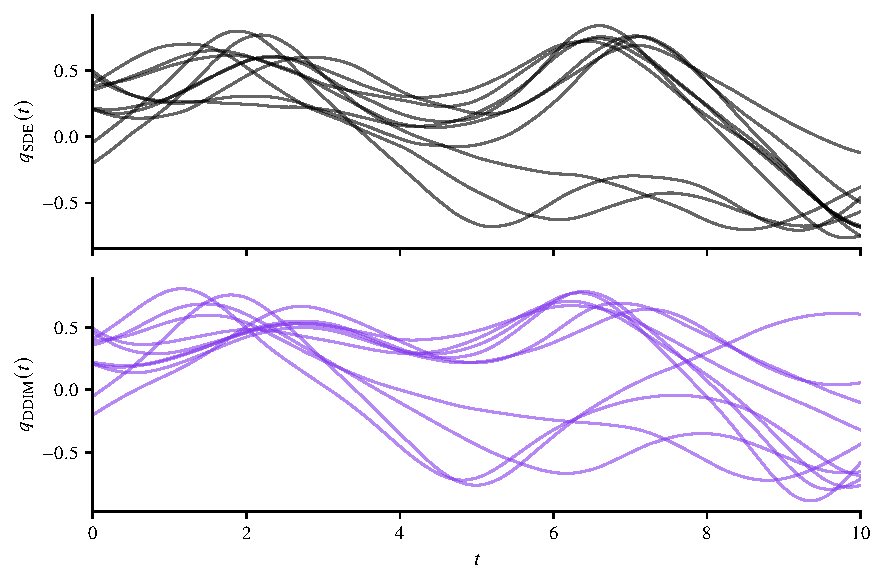
\includegraphics[width=\textwidth]{../do_trajectories.pdf}
    \caption{
    Representative held-out trajectories of the driven stochastic Duffing
    oscillator. Numerical trajectories obtained from the stochastic Heun solver
    are shown above and DDIM-generated trajectories below. Only the initial
    position $q(0)$ is supplied to the diffusion model; the initial velocity and
    both stochastic forcing terms remain unresolved. The generated ensemble
    reproduces the driven oscillatory response and the coexistence of
    dynamically distinct trajectories.
    }
    \label{fig:duffing_trajectories}
\end{figure}

Figure~\ref{fig:duffing_statistics} compares the corresponding ensemble statistics. The generated mean is almost indistinguishable from the numerical reference over the full trajectory, including the phase and amplitude of the driven oscillation. The one-standard-deviation intervals also overlap closely. The variance provides a more sensitive comparison. The model reproduces its rapid initial increase, the broad maximum near $t\simeq2$, the subsequent reduction around $t\simeq4$--$5$, and the later modulation. The first variance maximum is slightly underestimated, while the minimum near the centre of the interval is somewhat overestimated, but the overall time dependence is retained.

\begin{figure}[t]
    \centering
    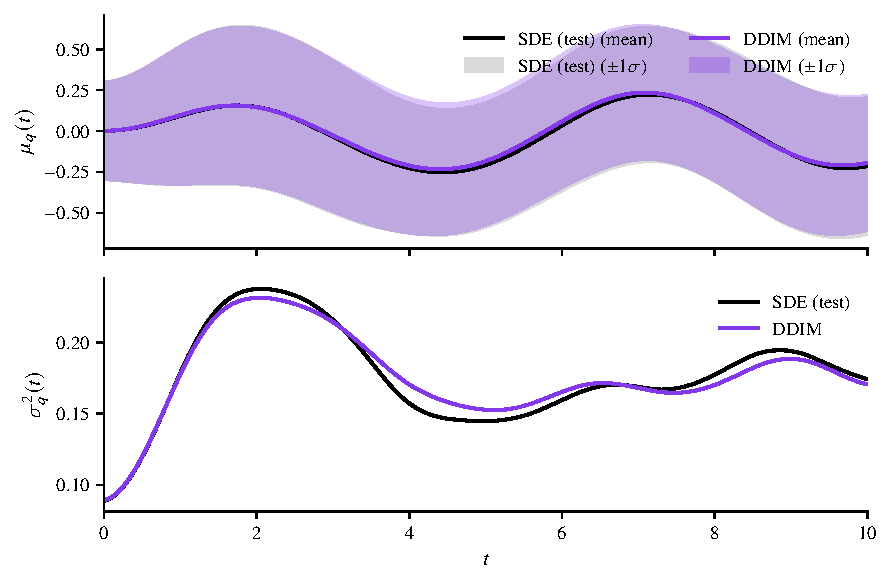
\includegraphics[width=\textwidth]{../do_statistics.pdf}
    \caption{
    Ensemble statistics for the held-out Duffing trajectories. The upper panel
    compares the time-dependent mean and one-standard-deviation interval of the
    stochastic numerical solver and the DDIM-generated ensemble. The lower
    panel compares their variances. The diffusion model reproduces the
    oscillatory mean response and the principal time dependence of the
    stochastic spread, including the initial variance growth and its subsequent
    modulation.
    }
    \label{fig:duffing_statistics}
\end{figure}

The Duffing example tests aspects of the conditional distribution that are absent from the OU process. The response is nonlinear, the stochastic forcing has both white and temporally correlated components, and the supplied condition does not specify the complete initial state. The close agreement of the ensemble statistics therefore indicates that the diffusion model can represent uncertainty associated with both stochastic dynamics and unresolved state variables.

% TODO: If available, add autocorrelation, power spectral density, pooled
% marginal distribution and Wasserstein-distance results here. These would test
% temporal and distributional structure beyond the first two moments.